\subsection{Luminosity} \label{sec:kaon_num}

\begin{figure}[htbp]
  \begin{tabular}{cc}
    \begin{minipage}{0.5\hsize}
      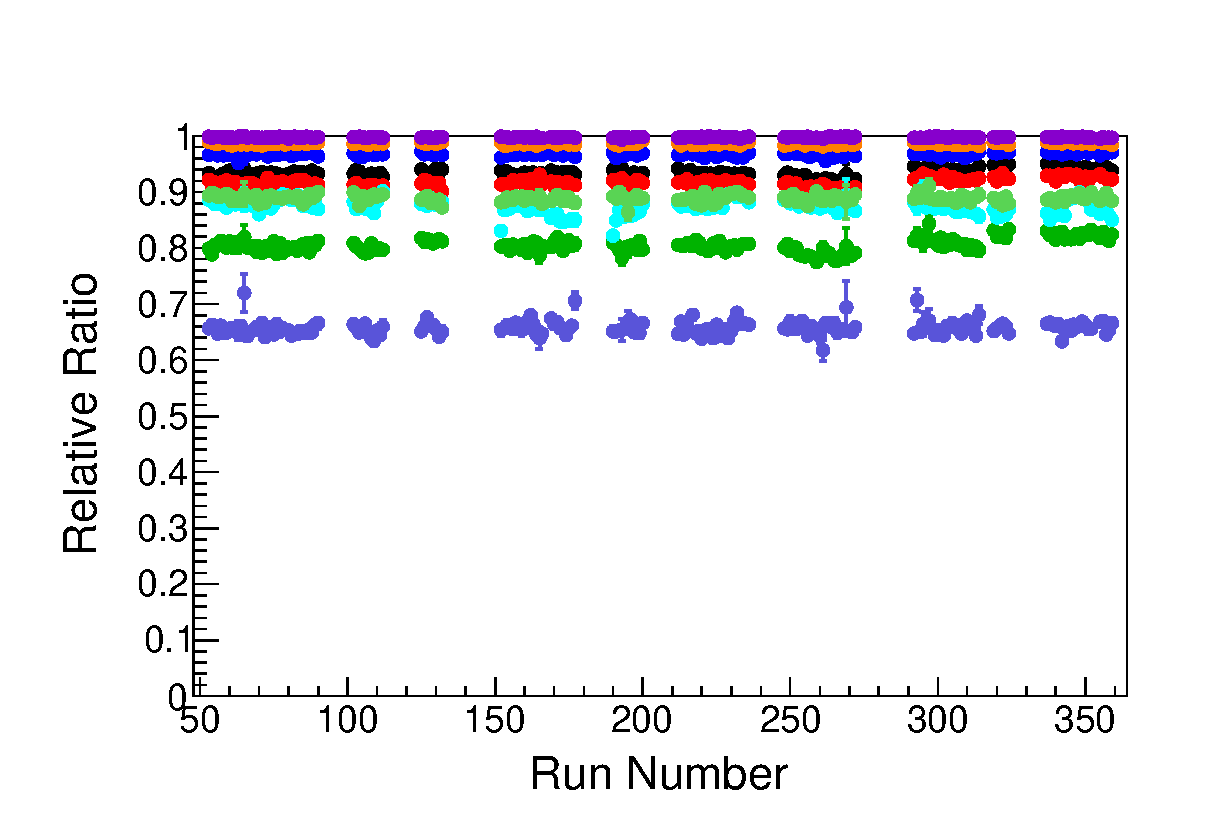
\includegraphics[width=6cm]{../pic/Run78/BL/relative_ratio.eps}
    \end{minipage}

    \begin{minipage}{0.5\hsize}
      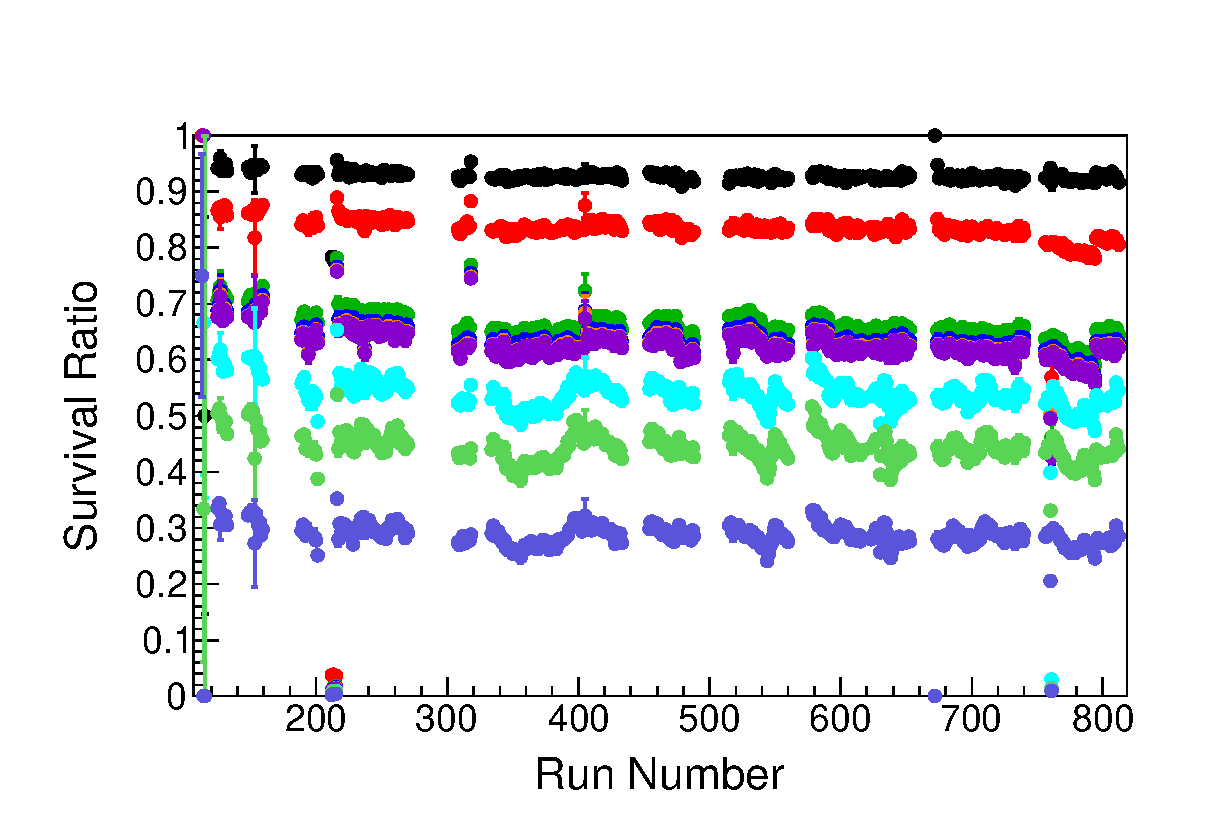
\includegraphics[width=6cm]{../pic/Run78/BL/survival_ratio.eps}
    \end{minipage}
  \end{tabular}
  \caption{
    Left and right figure indicates run dependence of relative and survival ratio in MR Run78, respectively.
    Relative ratio means ratio against before condition.
    Survival ratio means ratio from all K/f trigger events.
  }
  \label{fig:Kf_ratio}
\end{figure}

\begin{figure}[htbp]
  \centering
  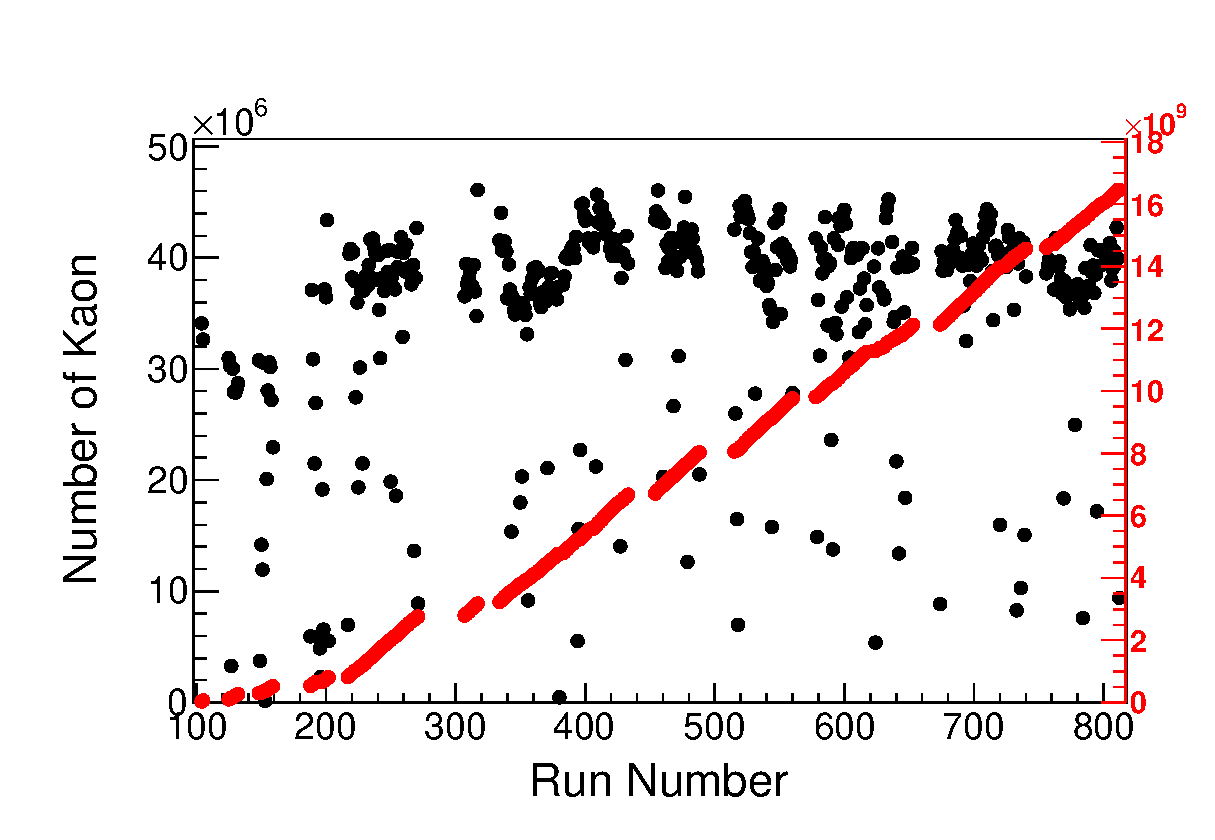
\includegraphics[width=8cm]{../pic/Run78/BL/Knum.eps}
  \caption{
    This figure shows kaon number irradiated on the liquid-$D_2$ target.
  }
  \label{fig:knum}
\end{figure}

The Kaon number of trigger levels is counted by the scaler DAQ, which also includes inaccurate events due to mixing of $pi$,
2-particles, and strange trajectories, as well as transformations and scattering on the beamline.
To avoid these events, a number of selections are made as described above. The following is a list of beamline selections.

\begin{enumerate}
\item T0 1hit selection
\item T0-BHD TOF kaon selection
\item BLC1 1track selection
\item BLC2 1track selection
\item D5 momentum reconstruction
\item D5 and BHD matching selection
\item BPC 1track selection
\item BLC2 and BPC connection
\item Beam on target at FF
\end{enumerate}   

These values is shown in Fig\ref{fig:Kf_ratio}.
Number of kaon irradiated on the liquid-$D_2$ target is shown in Figure.\ref{fig:knum}.
These values, together with the DAQ and trigger efficiencies described in the Section\ref{sec:trigger}, are evaluated as luminosity, as shown in the Table.\ref{tab:KP_scale} and \ref{tab:KN_scale}.
Data were collected on MR-Run69 for forward protons and MR-Run78 for forward neutrons.

\input{analysis/KP_scaling_table}
\input{analysis/KN_scaling_table}
